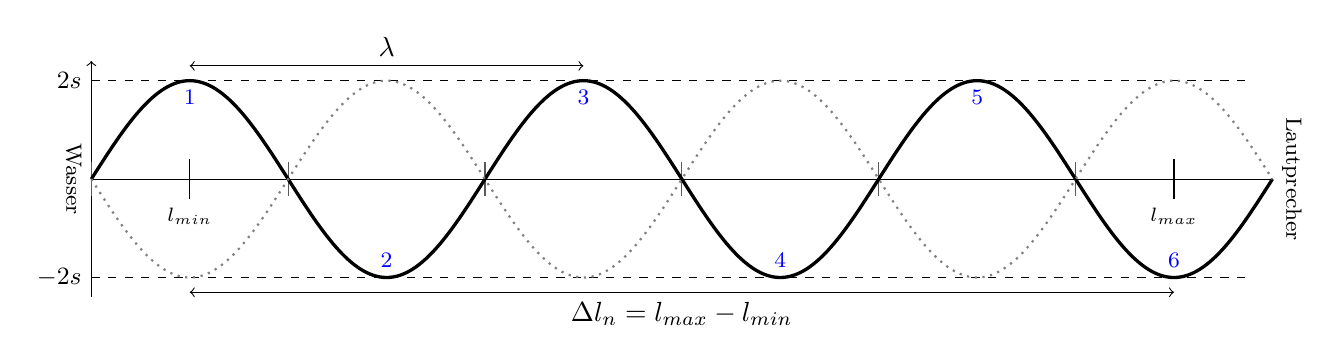
\begin{tikzpicture}[scale=1.25]
%    \begin{axis}[
%		xlabel=$x$,
%		ylabel={$f(x) = x^2 - x +4$}
%	]
%	% use TeX as calculator:
%	\addplot {sin(x)};
%	\end{axis}
    \draw node[below, rotate=-90,font=\footnotesize, fill=black!0, rounded corners]{Wasser}(0,0) -- (12,0) node[above, rotate=-90,font=\footnotesize, fill=black!0, rounded corners]{Lautprecher};
    \draw[dashed] (0,1)node[left,font=\small] {$2s$} -- (11.8,1); //obere Begrenzung
    \draw[dashed] (0,-1)node[left,font=\small] {$-2s$} -- (11.8,-1); //untere Begrenzung
    \draw[->](0,-1.2)--(0,1.2); // y-Pfeil
    \foreach \x in {0,2,...,10}{
    \draw[black!65] (\x,-0.17) -- (\x,0.17);
    }
    \draw[white,text=blue,font=\footnotesize] (0,0) -- ++(1,1) node[below]{1} -- ++(1,-1) -- ++(1,-1) node[above]{2} -- ++(1,1) -- ++(1,1) node[below]{3} -- ++(1,-1) -- ++(1,-1) node[above]{4} -- ++(1,1) -- ++(1,1) node[below]{5} -- ++(1,-1) -- ++(1,-1) node[above]{6} -- ++(1,1);
    \draw (1,0.2) -- (1,-0.2)node [below,font=\scriptsize,] {$l_{min}$};
    \draw (11,0.2) -- (11,-0.2)node [below,font=\scriptsize,] {$l_{max}$};
    \draw[<->] (1,1.15) -- node[above]{$\lambda$}(5,1.15);
    \draw[<->] (1,-1.15) -- node[below]{$\Delta l_n=l_{max}-l_{min}$}(11,-1.15);
    \draw[very thick] (0,0) sin ++(1,1) cos ++(1,-1) sin ++(1,-1) cos ++(1,1) sin ++(1,1) cos ++(1,-1) sin ++(1,-1) cos ++(1,1) sin ++(1,1) cos ++(1,-1) sin ++(1,-1) cos ++(1,1);   
     \draw[thick, dotted, black!50] (0,0) sin ++(1,-1) cos ++(1,1) sin ++(1,1) cos ++(1,-1) sin ++(1,-1) cos ++(1,1) sin ++(1,1) cos ++(1,-1) sin ++(1,-1) cos ++(1,1) sin ++(1,1) cos ++(1,-1);   
\end{tikzpicture}